\documentclass{beamer}
\usepackage{amsmath,amssymb,amsthm,graphicx}
\usepackage{color}
\usetheme{Gerrish}
\usepackage[mathcal]{euscript}   % for script letters
\usepackage{array}
\usepackage{bm}
\usepackage{wrapfig}
\usepackage{multirow}

\setbeamertemplate{navigation symbols}{}
\setbeamertemplate{outlinem}{}

\newcommand{\z}{\textbf{z}} 
\newcommand{\W}{\textbf{W}}
\newcommand{\mv}{\tilde{m}} 
\newcommand{\vv}[0]{\tilde{V}}
\newcommand{\w}{\textbf{w}}
\newcommand{\vphi}{\phi}
\newcommand{\bv}{\tilde{\beta}}
\newcommand{\bb}{\beta}
\newcommand{\lv}{\tilde{l}}
\newcommand{\vlv}{\sigma^2_{l}}
\newcommand{\vd}{\sigma^2_{d}}
\newcommand{\vbv}{\sigma^2}
\newcommand{\stdnorm}[1]{\mathcal{N}\left(#1\right)}


\newcommand{\tr}[0]{\mbox{Tr}}
\newcommand{\expectq}[1]{\mathbb{E}_q\left[#1\right]}
\newcommand{\expectqnoarg}[0]{\mathbb{E}_q}
\newcommand{\defn}[0]{:=}
\newcommand{\partl}[2]{\frac{\partial #1}{\partial #2}}


\title{A text-based model of foreign-affairs sentiment}
 \subtitle{} \date{17 December 2011} \author{Sean Gerrish and David Blei \\
   Princeton University Computer Science}

\begin{document}
\frame{\titlepage}

\frame {
 \frametitle{}
 \center
 
\includegraphics[width=0.9\textwidth]{figs/news.jpg} \\
 \LARGE
 \begin{center}
 These news articles tell a story.
 \end{center}
}

\frame {
 \frametitle{}
 \center
 
\includegraphics[width=1.0\textwidth]{figs/bad_headlines.jpg}
}

\frame {
 \frametitle{}
 \center
 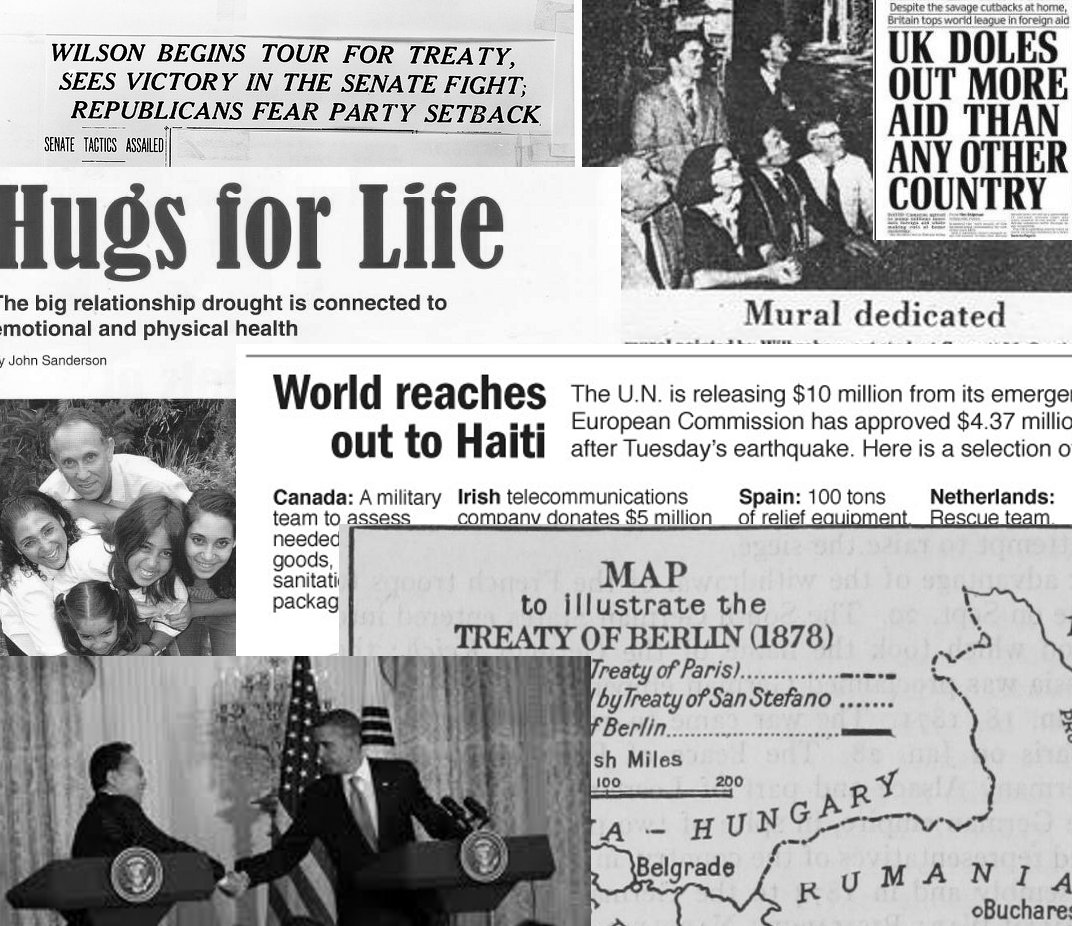
\includegraphics[width=1.0\textwidth]{figs/good_headlines.jpg}
}

\frame {
 \frametitle{A spatial model of foreign relations sentiment}
 \Large This work develops a model of the sentiment between countries over time.
 \begin{itemize}
   \item It models dynamic relationships in an interpretable way
   \item It infers sentiment from printed media
   \item Sentiment is defined by Mechanical Turkers
 \end{itemize}
}

\frame {
 \frametitle{A spatial model of foreign relations sentiment}
 \Large To do this, our plan is to:
 \begin{itemize}
   \item Collect a bunch of newspaper articles
   \item Define a latent variable model to capture interesting structure in these articles
   \item Perform posterior inference to estimate the value of these random variables
 \end{itemize}
}

\frame {
 \frametitle{Countries take latent positions $\bar x_{ct}$ over time}
 \center
 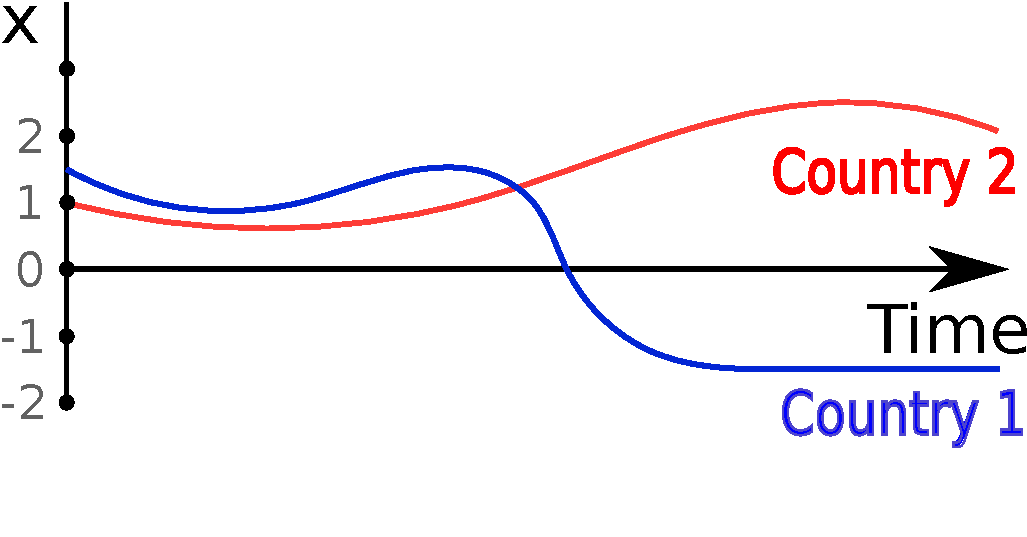
\includegraphics[width=0.8\textwidth]{figs/two_countries.pdf} \\
 \huge
 \begin{eqnarray*}
   \textcolor{blue}{\bar x_{c,t}} | \textcolor{blue}{\bar x_{c,t-1}} \sim N(\textcolor{blue}{\bar x_{c,t-1}}, \sigma_K^2) \nonumber \\
 \end{eqnarray*}
}

\frame {
 \frametitle{The relationship between countries is observed in the news.}
 \center
 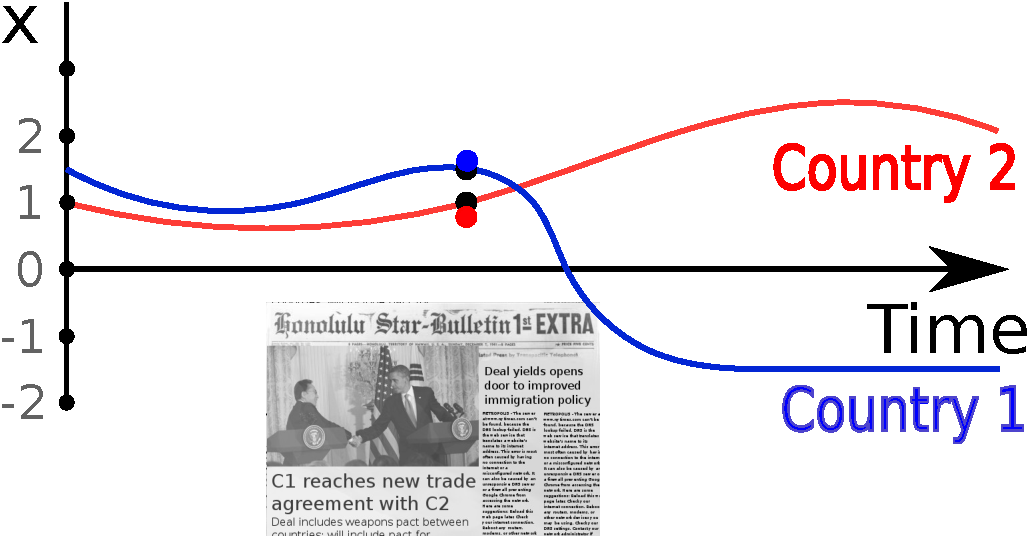
\includegraphics[width=0.8\textwidth]{figs/two_countries_time1.pdf}
 \center
 \LARGE
 \begin{eqnarray*}
  \textcolor{blue}{x_{c_1,d}} & \sim N(\textcolor{blue}{\bar x_{c_1, t}}, \sigma_D^2) \nonumber \\
  \textcolor{red}{x_{c_2,d}} & \sim N(\textcolor{red}{\bar x_{c_2, t}}, \sigma_D^2) \nonumber \\
  \mbox{Sentiment } s_d & := \textcolor{blue}{x_{c_1,d}}^T \textcolor{red}{x_{c_2,d}} \nonumber \\
 \end{eqnarray*}
}

\frame {
 \frametitle{The relationship between countries is observed in the news.}
 \center
 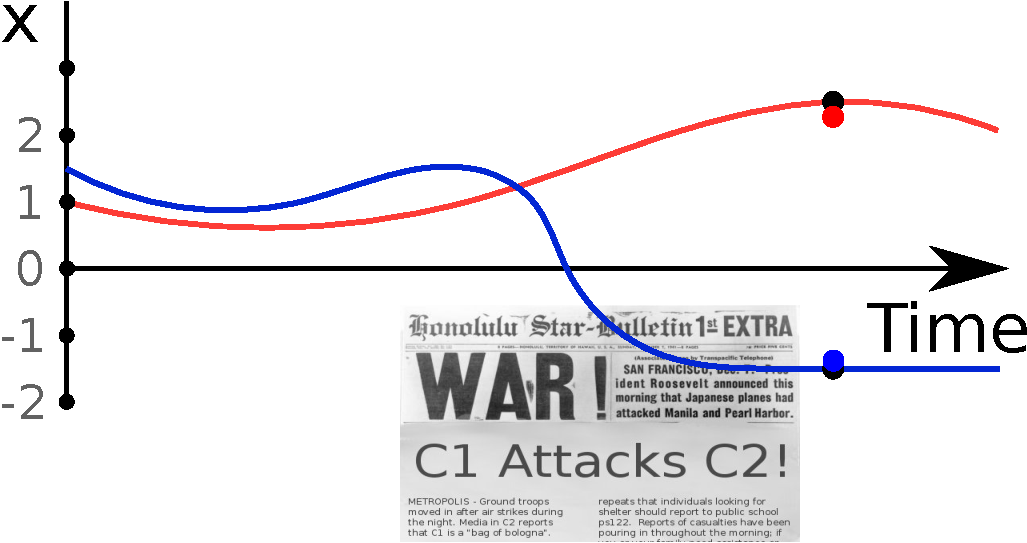
\includegraphics[width=0.8\textwidth]{figs/two_countries_time2.pdf}
 \LARGE
 \center
 \begin{eqnarray*}
  \textcolor{blue}{x_{c_1,d}} & \sim N(\textcolor{blue}{\bar x_{c_1, t}}, \sigma_D^2) \nonumber \\
  \textcolor{red}{x_{c_2,d}} & \sim N(\textcolor{red}{\bar x_{c_2, t}}, \sigma_D^2) \nonumber \\
  \mbox{Sentiment } s_d & := \textcolor{blue}{x_{c_1,d}}^T \textcolor{red}{x_{c_2,d}} \nonumber \\
 \end{eqnarray*}
}

\frame {
  \frametitle{The relationship between countries over time}
  \begin{center}
    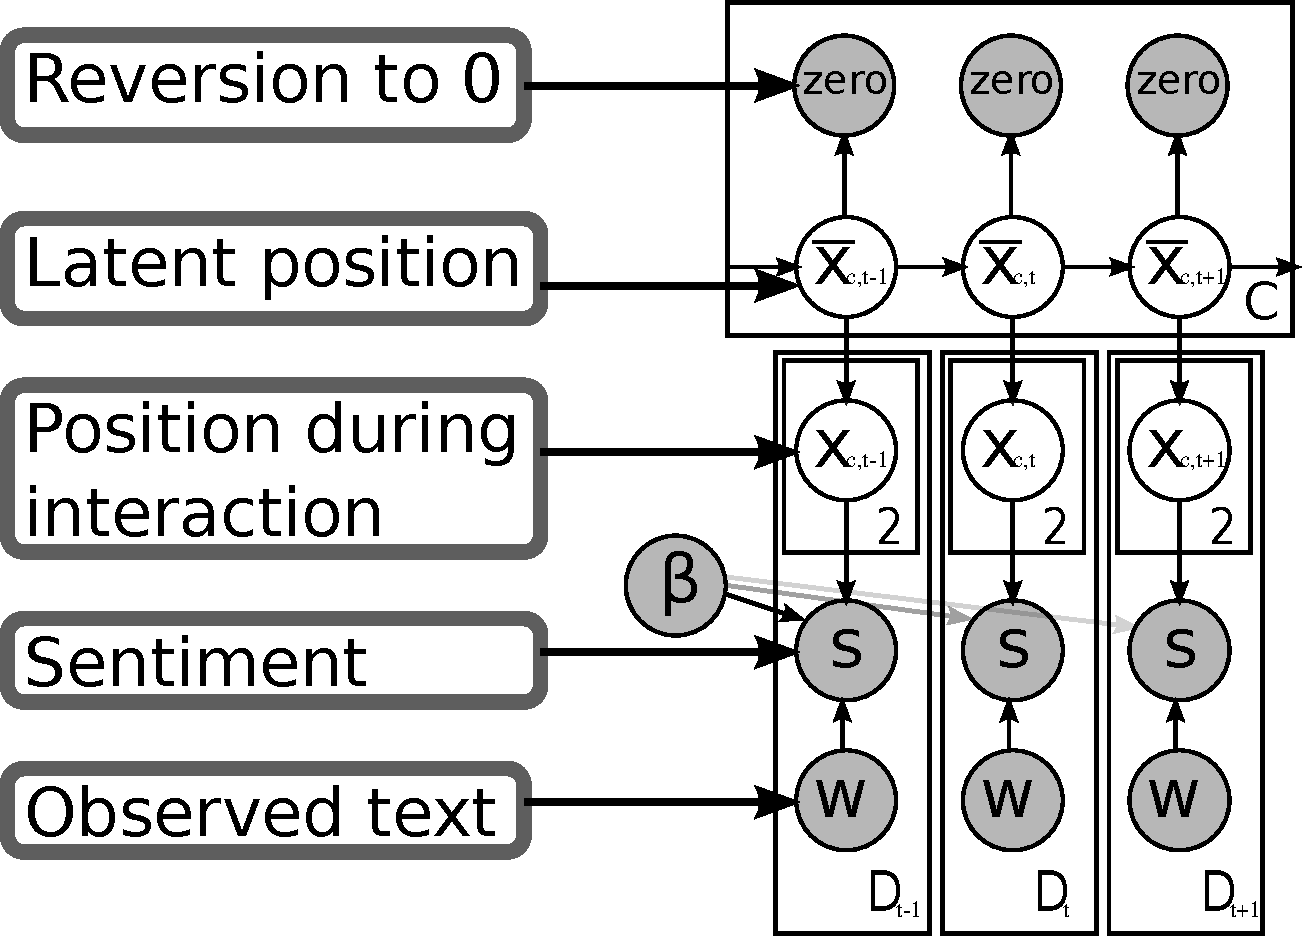
\includegraphics[height=0.8\textheight]{figs/countries_gm.pdf}
  \end{center}
}

\frame {
  \frametitle{Labeling sentiment}
  \center
  
\includegraphics{figs/amazon_mechanical_turk.jpg}
  \begin{enumerate}
  \item We found all pairs of paragraphs from the New York Times which
    discussed exactly two countries
  \item A random sample of 3607 paragraphs from \emph{New York Times} articles from 1988 to 2008 were labeled by Amazon Mechanical Turk workers
  \item Raters rated news articles on the scale $-5, -3, -1, 1, 3, 5$
  \end{enumerate}
}

\frame {
  \frametitle{Labeling sentiment: typical task}
  \center
  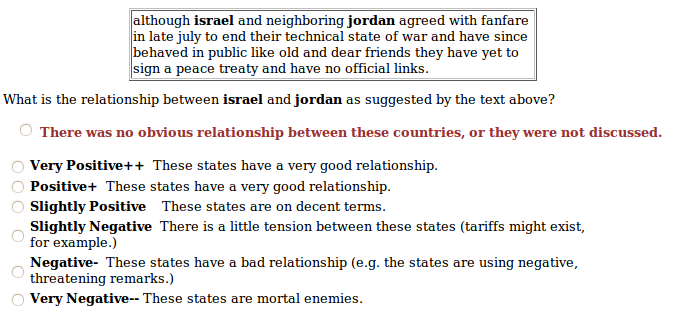
\includegraphics[width=1.1\textwidth]{figs/mturk_screenshot.png}
}

\frame {
 \frametitle{Sentiment and news articles: text regression}
 \huge
 \[
 s_d = \bm w_d^T \bm \beta + \varepsilon
 \]
 \Large
 \begin{itemize}
   \item $\bm w_d \in \mathbb{R}^V$ is the text of a news paragraph
   \item $s_d \in \mathbb{R}$ is the sentiment between two countries
   \item $\bm \beta \in \mathbb{R}^V$ is the ``weight'' of each word
 \end{itemize}
}

\frame {
 \frametitle{Sentiment and news articles: text parameter \LARGE $\beta$ }
 \hspace{-36pt}
 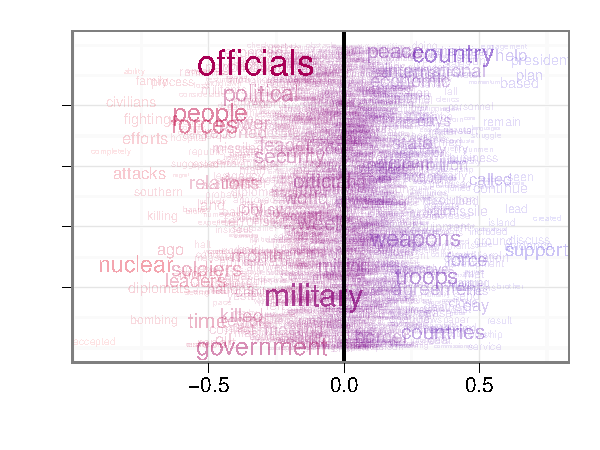
\includegraphics[width=1.1\textwidth]{figs/lm_sample_words.pdf}
}

\frame {
 \frametitle{Experiments}
 \begin{itemize}
 \item Randomly select 3607 paragraphs discussing pairs of 245 countries and territories.
  \item Label each of these paragraphs' sentiment with two ratings from Amazon Mechanical Turk.
  \item Hold out 42 random pairs (244 paragraphs) for testing.
  \item Fit sentiment model parameters $\beta$ on training paragraphs.
  \item Infer the spatial sentiment model with these parameters on all 257,472 paragraphs from 1988 to 2008.
%  \item Evaluate model sentiment prediction on the heldout 244 test
%    paragraphs.
 \end{itemize}
}

 \frame {
  \frametitle{Analysis with this model}
  To perform analysis with this model:
  \begin{enumerate}
    \item Fit the posterior (we used MAP)
    \item Inspect countries' means $\bar x_{c, \cdot}$
    \item Inspect the relationship between countries' means $\bar x_{c_1, t} \bar x_{c_2, t}$
  \end{enumerate}
 }

\frame {
 \frametitle{Results: selected countries' latent positions}
 \begin{tabular}{cc}
   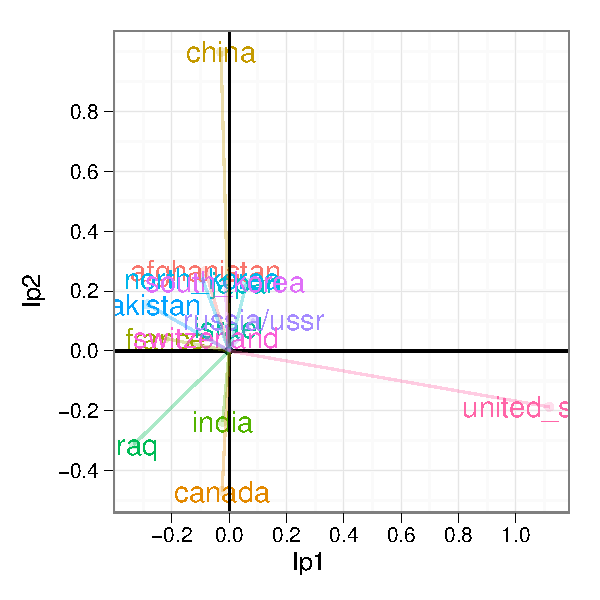
\includegraphics[width=0.5\textwidth]{figs/002_countries_by_ip_1987.pdf} &
   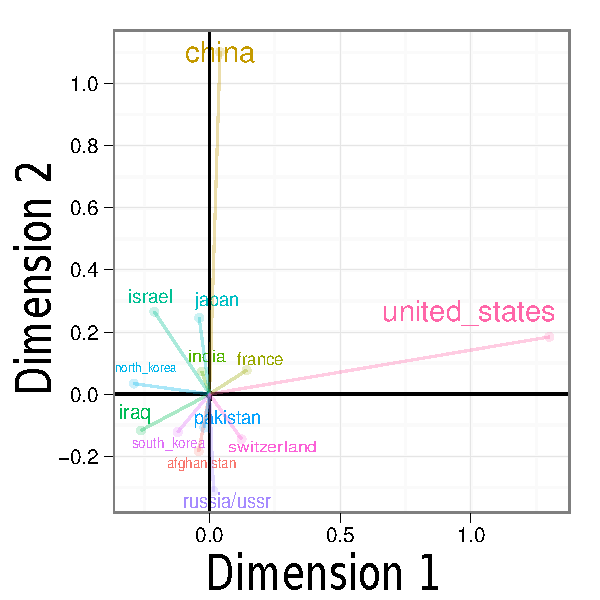
\includegraphics[width=0.5\textwidth]{figs/002_countries_by_ip_2007.pdf} \\
   \LARGE 1987 & \LARGE 2007 \\
 \end{tabular}
}

\frame {
 \frametitle{Results: selected countries' mutual sentiment with the U.S.}
 \begin{center}
 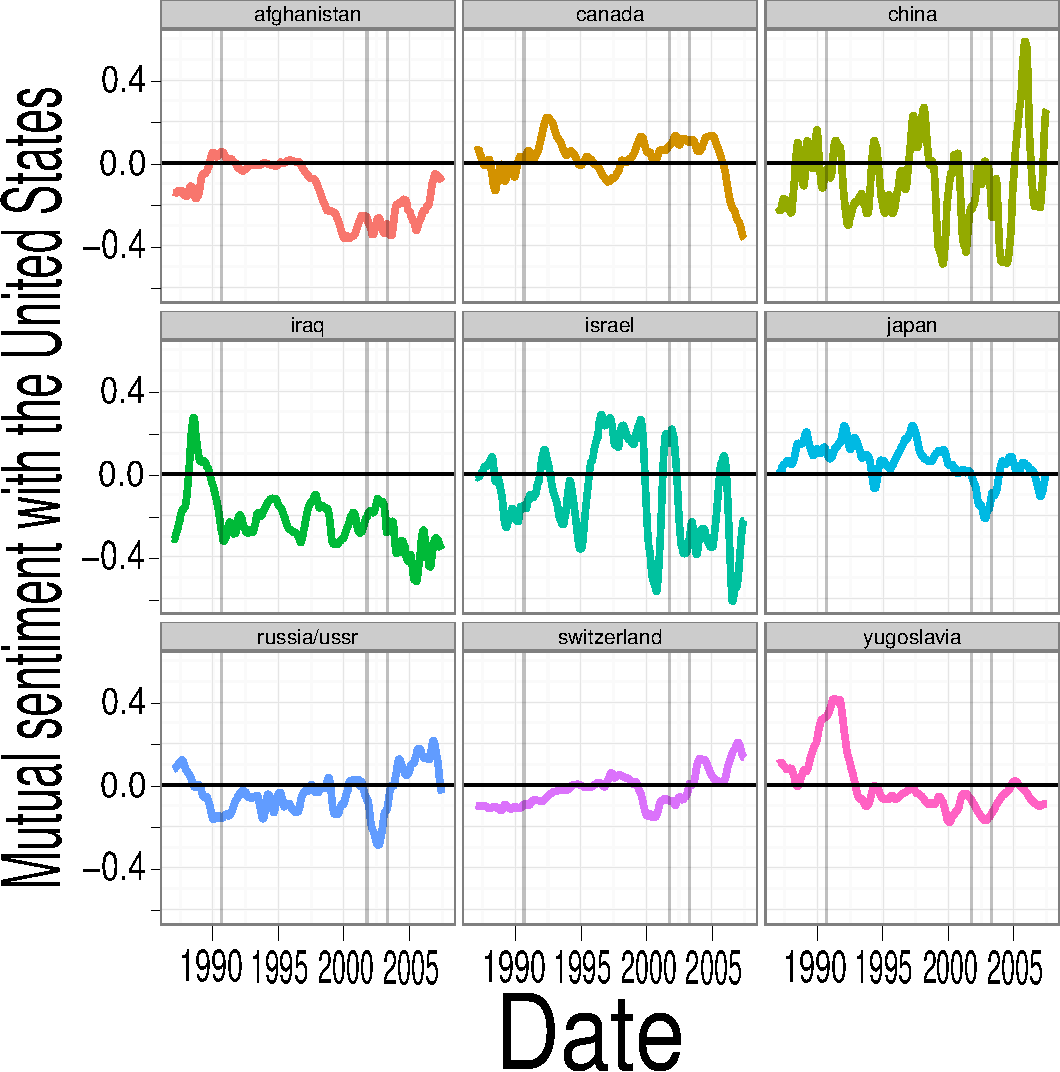
\includegraphics[height=0.8\textwidth]{figs/002_us_vs_everyone.pdf}
 \end{center}
}

\frame {
 \frametitle{Results: selected countries' mutual sentiment with Spain}
 \begin{center}
 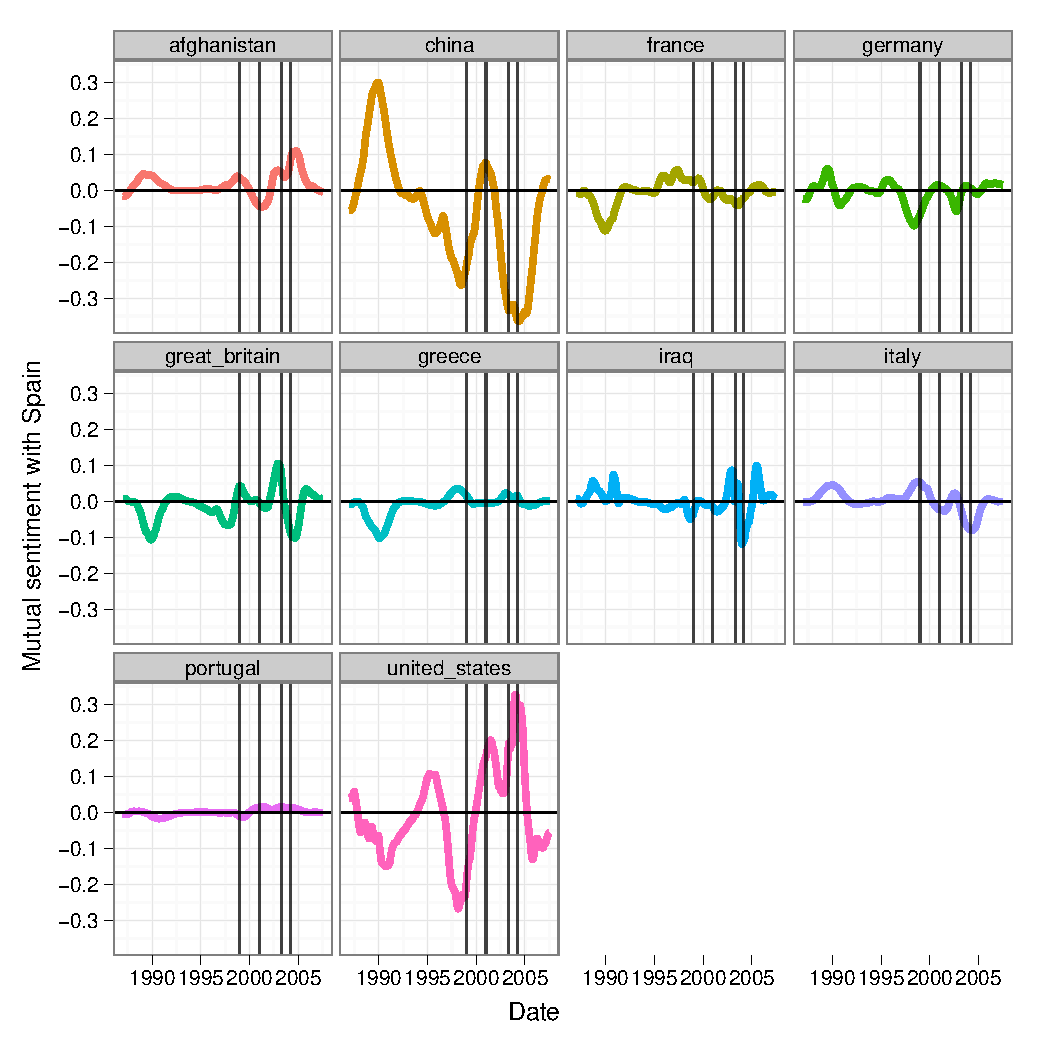
\includegraphics[height=0.8\textwidth]{figs/002_spain_vs_everyone.pdf}
 \end{center}
}

\frame {
 \frametitle{Evaluation}
 The model does better than text regression and individual \emph{Mechanical Turk} workers compared against one another.
 \begin{center}
   \hspace{-30pt} \begin{tabular}{|c|c|c|}
       \hline
       Model & Mean Squared Error & Mean Absolute Error \\
       \hline
       Inter-rater agreement & 1.77 (7.11) & 1.037 (2.07) \\
       \hline
       Text regression & 5.53 & 1.94 \\
       \hline
       Reversion variance 0.1 & 2.36 & 1.09 \\
       Reversion variance 1 & \textbf{2.32} & \textbf{1.07} \\
       Reversion variance 10 & 2.32 & 1.08 \\
       Reversion variance 100 & 2.34 & 1.09 \\
       Reversion variance 1000 & 2.33 & 1.08 \\
       \hline
     \end{tabular}
     \label{figure:sse_test}
   \end{center}
}

\frame{
  \frametitle{Current work and future directions}
  \begin{itemize}
  \item Sentiment intercepts for each country
  \item Infer asymmetric relationships
  \item Application to other dyads
  \item Infer unsupervised relations
    \begin{itemize}
    \item Sentiment is only one dimension
    \item Similar to relational topic models \cite{chang:2009}
    \end{itemize}
  \end{itemize}
}

\frame{
  \frametitle{Thank you}
  \begin{itemize}
    \item Sean Gerrish (sgerrish@cs.princeton.edu)
    \item David Blei (blei@cs.princeton.edu)
  \end{itemize}
}
%%% Local Variables: 
%%% mode: latex
%%% TeX-master: "talk"
%%% End: 
\small
\bibliographystyle{nips}
\small

\frame{
\frametitle{Bibliography}
\bibliography{../bib}
}

\end{document}
